% !TeX root = ../main.tex
% This is section 6.

\section{分离性}

\subsection{分离性公理}

    分离性主要体现拓扑空间中点与点或点与集合能否被有效地分开, 它引出以下的问题: 序列的极限是否唯一? 网的极限是否唯一?

    \begin{Definition}[$ T_0,T_1,T_2 $公理]
        设 $ (X,\ST) $ 是一个拓扑空间, 对任意 $ x,y\in X $ 且 $ x\ne y $:
        \begin{enumerate}
            \item 若两点中有一个点存在一个邻域不包含对方, 即
            \[
                \forall x,y\in X,\, x\ne y\,(\exists U_x\in\CN(x)\,(y\notin U_x)\lor(\exists U_y\in\CN(y)\,(x\notin U_y))),
            \]
            则称 $ X $ 满足 $ T_0 $\emph{公理}, 或 $ X $ 是 $ T_0 $\emph{空间}.
            \item 若两点各存在一个邻域不包含对方, 即
            \[
                \forall x,y\in X,\, x\ne y\,(\exists U_x\in\CN(x)\,(y\notin U_x)\land(\exists U_y\in\CN(y)\,(x\notin U_y))),
            \]
            则称 $ X $ 满足 $ T_1 $\emph{公理}, 或 $ X $ 是 $ T_1 $\emph{空间}.
            \item 若两点各存在一个邻域, 使得两邻域不交, 即
            \[
                \forall x,y\in X,\, x\ne y\,\exists U_x\in\CN(x)\,\exists U_y\in\CN(y)\,(U_x\cap U_y=\varnothing),
            \]
            则称 $ X $ 满足 $ T_2 $\emph{公理}, 或 $ X $ 是 $ T_2 $\emph{空间}, 有时也称作 \emph{Hausdorff 空间}.
        \end{enumerate}
    \end{Definition}

    \begin{figure*}[!htb]
        \centering
        \subfloat[$ T_0 $空间]{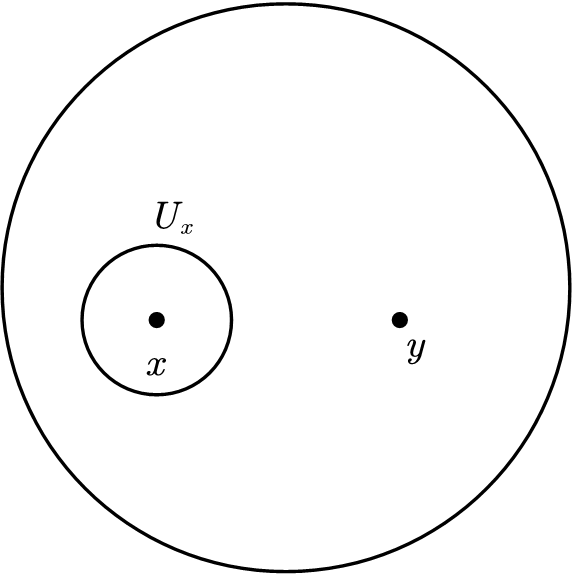
\includegraphics[width=0.2\linewidth]{figures/T0_1.png} 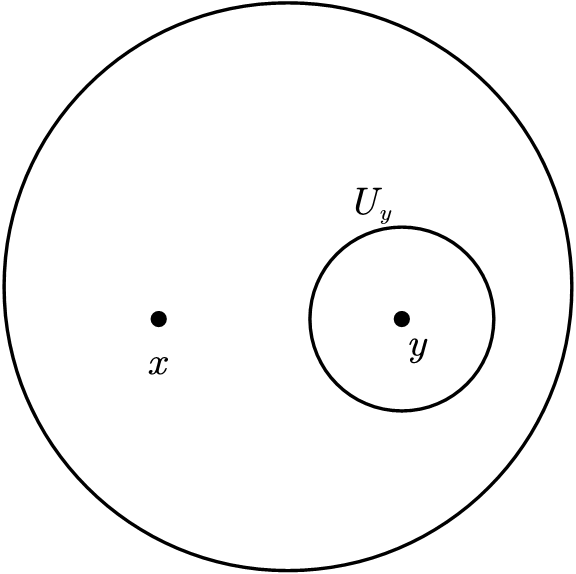
\includegraphics[width=0.2\linewidth]{figures/T0_2.png}} \quad \subfloat[$ T_1 $空间]{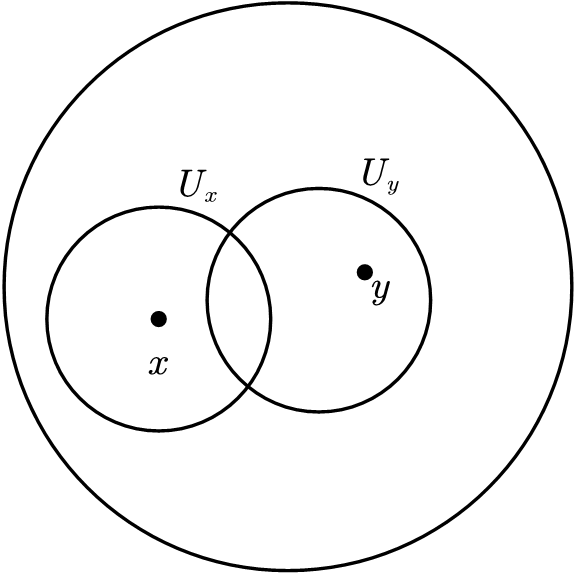
\includegraphics[width=0.2\linewidth]{figures/T1.png}} \quad \subfloat[$ T_2 $空间]{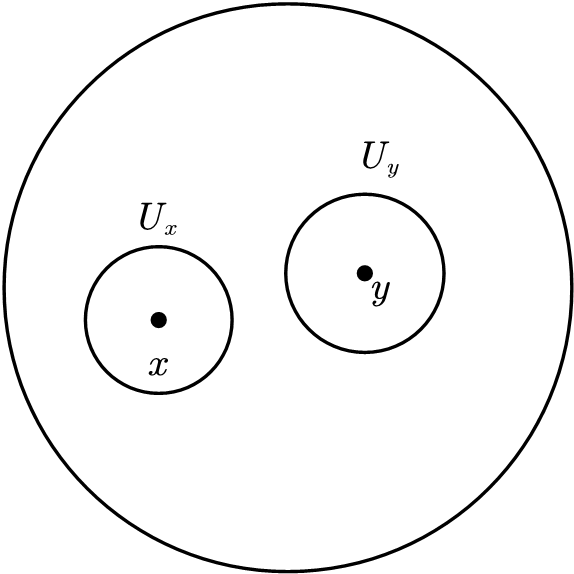
\includegraphics[width=0.2\linewidth]{figures/T2.png}}
        %\caption{ $ T_0,T_1,T_2 $ 分离性公理的图示 }
    \end{figure*}

    由定义可知 $ T_2 $ 空间一定是 $ T_1 $ 的, $ T_1 $ 空间一定是 $ T_0 $ 的.

    仅靠邻域来描述分离性往往不便于实际使用, 为此给出一些等价刻画:

    \begin{Proposition}[$ T_0 $空间的刻画]
        $ X $ 是 $ T_0 $ 空间当且仅当 $ \forall x,y\in X\,(x\ne y\Rightarrow\baro{\set{x}}\ne\baro{\set{y}}) $.
    \end{Proposition}
    \begin{Proof}
        \textsl{必要性}. 若 $ X $ 是 $ T_0 $ 空间, 不妨设存在 $ x $ 的邻域 $ U_x $ 使得 $ y\notin U_x $, 则
        \[
            U_x\cap\set{y}=\varnothing\Longleftrightarrow U_x\cap(\set{y}\sm\set{x})=\varnothing\Longrightarrow x\notin\baro{\set{y}},
        \]
        故 $ \baro{\set{x}}\ne\baro{\set{y}} $.

        \textsl{充分性}. 因对任意不同的 $ x,y\in X $, 都有 $ \baro{\set{x}}\ne\baro{\set y} $, 不妨设 $ \baro{\set{x}}\subset\baro{\set{y}} $ 不成立, 于是
        \[
            x\notin\baro{\set{y}}\Longleftrightarrow x\in\baro{\set{y}}^c,
        \]
        令 $ U=\baro{\set{y}}^c\in\CN(x) $ 即可.\qed
    \end{Proof}

    \begin{Proposition}[$ T_1 $空间的刻画]
        $ X $ 是 $ T_1 $ 空间当且仅当 $ X $ 中的单点集都是闭集.
    \end{Proposition}
    \begin{Proof}
        \textsl{必要性}. 设 $ X $ 是 $ T_1 $ 空间, $ x_0\in X $, 只需证明 $ X\sm\set{x_0} $ 是开集. 由 $ X $ 是 $ T_1 $ 的可知
        \[
            \forall x\in X\sm\set{x_0}\,\exists U\in\CN(x)\,(x_0\notin U),
        \]
        即 $ x\in U\subset X\sm\set{x_0} $, 这说明 $ x $ 是 $ X\sm\set{x_0} $ 的内点, 于是 $ X\sm\set{x_0} $ 是开集.

        \textsl{充分性}. 因为 $ X $ 中的单点集都是闭集, 于是对任意不同的 $ x,y\in X $, 有 $ X\sm\set{x} $ 和 $ X\sm\set{y} $ 是开集, 且
        \[
            (x\in X\sm\set{y},\ y\notin X\sm\set{y})\land(y\in X\sm\set{x},\ x\notin X\sm\set{x})
        \]
        恒真, 由 $ X\sm\set{x}\in\CN(y) $ 和 $ X\sm\set{y}\in\CN(x) $ 可知 $ X $ 是 $ T_1 $ 的.\qed
    \end{Proof}

    借助所谓的``特殊化序''的工具可以将上面的刻画换一种说法来表述: 在 $ X $ 中定义一个二元关系 $ x \lesssim y $ 当且仅当 $ x\in\baro{\set{y}} $, 这一关系满足自反性和传递性, 从而是一个准序, 这一关系称作 $ X $ 上的特殊化序. 因此 $ X $ 是 $ T_0 $ 的当且仅当 $ X $ 上的特殊化序是偏序, 而 $ X $ 是 $ T_1 $ 的当且仅当 $ X $ 上的特殊化序是相等.

    \begin{Proposition}[$ T_2 $空间的刻画]
        $ X $ 是 $ T_2 $ 空间当且仅当 $ X $ 中的网极限唯一.
    \end{Proposition}
    \begin{Proof}
        \textsl{必要性}. 用反证法, 不妨设 $ \alpha $ 是一上定向集, 若极限不唯一, 即存在 $ X $ 中的网 $ (x_i)_{i\uparrow\alpha} $ 使得 $ \lim_{i\uparrow\alpha}x_i=a $ 且 $ \lim_{i\uparrow\alpha}x_i=b $ 满足 $ a\ne b $. 因 $ X $ 是 $ T_2 $ 的, 故存在 $ U_a\in\CN(a) $, $ U_b\in\CN(b) $ 使得 $ U_a\cap U_b=\varnothing $. 而由极限的定义, 有
        \[
            \begin{aligned}
                \lim_{i\uparrow\alpha}x_i=a\Longleftrightarrow\exists n_1\in\alpha\forall n\geqslant n_1\,(x_n\in U_a) \\
                \lim_{i\uparrow\alpha}x_i=b\Longleftrightarrow\exists n_2\in\alpha\forall n\geqslant n_2\,(x_n\in U_b)
            \end{aligned}
        \]
        而 $ \alpha $ 是上定向的, 于是存在 $ m\in\alpha\,(m\geqslant n_1\land m\geqslant n_2) $, 于是 $ x_m\in U_a\cap U_b $, 矛盾.
        
        \textsl{充分性}. 依然使用反证法, 若 $ X $ 不是 $ T_2 $ 的, 则存在 $ x\ne y $ 使得它们的开邻域交集恒非空. 考虑所有开邻域对 $ (U_i, V_j) $ 在包含关系下构成的有向集合(它显然上定向)并令 $ z_{i,j}\in U_i\cap V_j $, 则 $ z_{i,j}\to x $ 且 $ z_{i,j}\to y $, 矛盾.\qed
    \end{Proof}

    特别地, 对 $ T_1 $ 空间中的聚点, 有以下的刻画:
    \begin{Proposition}
        设 $ X $ 是 $ T_1 $ 空间, $ x\in X,\ A\subset X $, 则
        \[
            x\in d(A)\Longleftrightarrow\forall U\in\CN(x)\,(\abs{U\cap A}=\infty).
        \]
    \end{Proposition}
    \begin{Proof}
        \textsl{必要性}. 因 $ x\in d(A) $, 若存在 $ U\in\CN(x) $ 使得 $ U\cap A $ 有限, 取 $ B=U\cap(A\sm\set{x}) $ 也是有限集. 由 $ X $ 是 $ T_1 $ 空间可知 $ B $ 是闭集, 于是 $ U\sm B $ 是开的, 从而 $ U\sm B\in\CN(x) $. 但
        \[
            (U\sm B)\cap(A\sm\set{x})=(U\cap(A\sm\set{x}))\sm B=B\sm B=\varnothing,
        \]
        即 $ x\notin d(A) $, 矛盾.
        
        \textsl{充分性}. 显然成立.\qed
    \end{Proof}

    \begin{Example}
        下面的例子是容易验证的:
        \begin{enumerate}
            \item 多于一点的平凡拓扑空间都不是 $ T_0 $ 的.
            \item 在实直线 $ \R $ 上赋予\emph{右拓扑} $ \ST_R:=\set{(a,\infty) : a\in\R} $ 后的拓扑空间 $ (\R,\ST_R) $ 是 $ T_0 $ 的, 但不是 $ T_1 $ 的.
            \item 含有无限多个点的有限补空间都是 $ T_1 $ 但非 $ T_2 $ 的. 因有限集均为闭集, 单点集必为闭集, 从而 $ X $ 是 $ T_1 $ 的. 但任取 $ X $ 中的两个非空开集 $ O_1,O_2\in\ST $ 后 $ O_1^c,\ O_2^c $ 都是有限集, 注意到
            \[
                O_1\cap O_2=(O_1^c\cup O_2^c)^c,
            \]
            由 $ X $ 是无限集可知 $ O_1\cap O_2 $ 也是无限集, 即 $ O_1\cap O_2\ne\varnothing $, 于是 $ X $ 不可能是 $ T_2 $ 的.
            \item 在实直线 $ \R $ 上赋予通常的拓扑构成的拓扑空间是 $ T_2 $ 的.
        \end{enumerate}
    \end{Example}

    \begin{Example}
        含有无限多个点的有限补空间中的序列可能存在无限多个极限点, 不妨取 $ (x_n)_{n\geqslant 1}\subset X $ 满足对任意 $ i\ne j $ 有 $ x_i\ne x_j $. 任取 $ y\in X $ 和 $ U\in\CN(y) $. 因 $ U^c $ 有限, 于是 $ (x_n)_{n\geqslant 1} $ 中至多有限项落在 $ U^c $ 中, 于是
        \[
            \exists n_0\in\Zi\,(n>n_0\Rightarrow x_n\in U),
        \]
        即 $ \lim_{n\to\infty}x_n=y $. 由 $ y $ 的任意性可知 $ X $ 中任意一点都是序列 $ (x_n)_{n\geqslant 1} $ 的极限.
    \end{Example}

\subsection{正则性和正规性}

    本小节开始不仅讨论点和点的分离性, 也开始讨论点和集合的分离性. 为此引入集合的邻域系:

    \begin{Definition}[集合的邻域系]
        设 $ A\subset X $, 若 $ \forall x\in A\,(U\in\CN(x)) $, 则称 $ U $ 是 $ A $ 的一个\emph{邻域}. $ A $ 的邻域全体 $ \CN(A) $ 称作 $ A $ 的\emph{邻域系}. 若 $ U $ 还是一个开集, 则称 $ U $ 是 $ A $ 的开邻域.
    \end{Definition}

    在这里约定, 以后取邻域总假设取到的是开邻域.

    \begin{Definition}[正则公理, 正规公理]
        设 $ X $ 是一拓扑空间:
        \begin{enumerate}
            \item 若对一个点和一个闭集, 它们各存在一个邻域使得这两个邻域不交, 即
            \[
                \forall F\in\SF\,\forall x\notin F\,\exists U\in\CN(x)\,\exists V\in\CN(F)\,(U\cap V=\varnothing)
            \]
            则称 $ X $ 是\emph{正则空间}.
            \item 若对两个闭集, 它们各存在一个邻域使得这两个邻域不交, 即
            \[
                \forall F_1,F_2\in\SF\,\exists U\in\CN(F_1)\,\exists V\in\CN(F_2)\,(U\cap V=\varnothing)
            \]
            则称 $ X $ 是\emph{正规空间}.
        \end{enumerate}
    \end{Definition}

    注意正则和正规是互不蕴含的, 并且它们与之前提到的 $ T_0 $ 公理和 $ T_1 $ 公理也互不蕴含, 因为一般拓扑空间上的单点集不可以被认为是闭集. 下面给出了一个非 $ T_0 $ 却正则且正规的例子:

    \begin{Example}
        取 $ X=\set{1,2,3} $, $ \ST=\set{\varnothing,\set{1},\set{2,3},X} $, 则 $ (X,\ST) $ 是既正则又正规的拓扑空间, 但 $ 2\ne 3 $ 而 $ \baro{\set{2}}=\baro{\set{3}}=\set{2,3} $, 故 $ (X,\ST) $ 不是 $ T_0 $ 的, 自然也不是 $ T_1 $ 或 $ T_2 $ 的.
    \end{Example}

    \begin{Proposition}[正则空间的刻画]\label{prop:正则空间的刻画}
        $ X $ 是正则空间当且仅当 $ \forall x\in X\,\forall U\in\CN(x)\,\exists V\in\CN(x)\,(\bar{V}\subset U) $.
    \end{Proposition}
    \begin{Proof}
        \textsl{必要性}. 任取 $ x\in X $, $ U\in\CN(x) $, 则 $ U^c $ 是闭集, $ x\notin U^c $. 由 $ X $ 的正则性可知
        \[
            \exists U_1\in\CN(x)\,\exists V_1\in\CN(U^c)\,(U_1\cap V_1=\varnothing),
        \]
        故 $ U_1\subset V_1^c $. 对两侧取闭包可知 $ \baro{U_1}=\baro{V_1}^c=V_1^c\subset U $, 取 $ V=U_1 $ 即可.
        
        \textsl{充分性}. 对任意 $ x\in X $ 和 $ F\in\SF $ 使得 $ x\notin F $, 都有 $ F^c $ 是开集, 且 $ x\in F^c $, 从而 $ F^c\in\CN(x) $. 由题设可知存在 $ U\in\CN(x) $ 使得 $ \bar{U}\subset F^c $, 令 $ V=\bar{U}^c $ 后 $ V $ 是开集, 且
        \[
            F\subset\bar{U}^c=V=\mathring{V}.
        \]
        即 $ V\in\CN(F) $, 且 $ U\cap V=\varnothing $, 也即 $ X $ 是正则的.\qed
    \end{Proof}

    \begin{Proposition}[正规空间的刻画]
        $ X $ 是正规空间当且仅当 $ \forall F\in\SF\,\forall U\in\CN(F)\,\exists V\in\CN(F)\,(\bar{V}\subset U) $.
    \end{Proposition}
    \begin{Proof}
        与命题 \ref{prop:正则空间的刻画} 类似可证.\qed
    \end{Proof}

    为了研究更强的分离性, 不但需要要求点和点之间可以良好地分离, 还要求点和集合之间可以良好地分离. 这显然是一种更强的分离性:

    \begin{Definition}[$ T_3,T_4 $公理]
        设 $ (X,\ST) $ 是 $ T_1 $ 空间. 若 $ X $ 还是正则的, 则称 $ X $ 是 $ T_3 $ \emph{空间}; 若 $ X $ 还是正规的, 则称 $ X $ 是 $ T_4 $ \emph{空间}.
    \end{Definition}

    因 $ T_1 $ 空间中的单点集就是闭集, 于是 $ T_4 $ 空间一定是 $ T_3 $ 的, $ T_3 $ 空间一定是 $ T_2 $ 的.

    \begin{Theorem}
        度量空间是 $ T_4 $ 空间.
    \end{Theorem}
    \begin{Proof}
        易知度量空间是 $ T_1 $ 的, 只需证明它正规. 为此取 $ A, B\in\SF $ 使得 $ A\cap B=\varnothing $, 则对任意 $ x\in F_1 $ 使得 $ d(x,B)>0 $, 取
        \[
            U=\bigcup_{x\in A}B\left(x,\frac{d(x,B)}{2}\right),\quad V=\bigcup_{x\in B}B\left(x,\frac{d(x,A)}{2}\right),
        \]
        易知 $ U\in\CN(A) $, $ V\in\CN(B) $ 且 $ U\cap V=\varnothing $. 这因 $ \forall x\in A,\ \forall y\in B,\ \forall z\in U\cap V $ 有
        \[
            d(x,y)\leqslant d(x,z)+d(y,z)<\frac{1}{2}(d(x,B)+d(y,A))\leqslant\frac{1}{2}(d(x,y)+d(y,x))=d(x,y),
        \]
        矛盾.\qed
    \end{Proof}

    \begin{Proposition}
        分离性是拓扑性质.
    \end{Proposition}

    \begin{Proposition}
        以下 $ i=0,1,2,3 $, $ T_i $(或正则)空间的子空间和有限集空间仍然是 $ T_i $(或正则)空间; 但 $ T_4 $(或正规)空间的子空间或有限积空间未必是 $ T_4 $(或正规)空间.
    \end{Proposition}

    下面给出一个 $ T_4 $ 空间的子空间非 $ T_4 $ 的例子, 有限积空间的反例有些复杂, 此处不再进一步讨论.

    \begin{Example}
        考虑 $ X=\set{a,b,c,d} $, 在其上取拓扑 $ \ST=\set{\varnothing,\set{b},\set{a,b},\set{b,c},\set{a,b,c},X} $. 在这一拓扑空间上非空闭集一定包含 $ d $, 从而必定两两相交; 故若存在两个不交的闭集, 它们必有之一是空集, 于是 $ X $ 是 $ T_4 $ 的.
        
        再考虑其子空间拓扑 $ Y=\set{a,b,c} $, $ \tilde{\ST}=\ST|_Y $. 此时存在不交闭集 $ \set{a} $ 和 $ \set{c} $, 其中 $ \set{a} $ 的开邻域只有 $ \set{a,b} $ 和 $ Y $, $ \set{c} $ 的开邻域只有 $ \set{b,c} $ 和 $ Y $. 其开邻域均含有 $ b $, 不可能不交, 于是子空间拓扑不是 $ T_4 $ 的.
    \end{Example}

    下面的图表说明了分离性公理之间的联系:

    \begin{center}
        \begin{tikzpicture}
            \node (D) at (-4,0) {度量空间};
            \node (T4) at (-2,0) {$ T_4 $};
            \node (T3) at (-0.5,0) {$ T_3 $};
            \node (T2) at (1,0) {$ T_2 $};
            \node (T1) at (2.5,0) {$ T_1 $};
            \node (T0) at (4,0) {$ T_0 $};
            \node (Nor) at (-2,-1.2) {正规};
            \node (R) at (-0.5,-1.2) {正则};
            \draw[->] (D) -- (T4);
            \draw[->] (T4) -- (T3);
            \draw[->] (T3) -- (T2);
            \draw[->] (T2) -- (T1);
            \draw[->] (T1) -- (T0);
            \draw[->] (T4) -- (Nor);
            \draw[->] (T3) -- (R);
        \end{tikzpicture}
    \end{center}

\subsection{可度量化空间}

    相较于度量空间, 拓扑空间实际上就是从度量空间中剥离了度量结构. 事实上, 我们并不能将连续映射作为度量空间的结构映射, 因为它不保距. 度量空间的连续映射给出了度量空间作为拓扑空间的结构映射, 而度量空间的结构映射是保距映射. 一个小彩蛋是, 足够好的拓扑空间是可以在其上定义度量, 使该度量诱导的拓扑与原拓扑相同的.

    \begin{Definition}[可度量化空间]
        若 $ X $ 上的拓扑 $ \ST $ 可以被度量 $ d $ 诱导, 则称 $ (X,\ST) $ 是\emph{可度量化}的.
    \end{Definition}

    下面的命题说明可数性可以对分离性产生影响:

    \begin{Proposition}
        满足 $ C_2 $ 公理的 $ T_3 $ 空间是 $ T_4 $ 空间.
    \end{Proposition}
    \begin{Proof}
        设 $ X $ 有可数拓扑基 $ \CB $, 且由 $ T_3 $ 公理可知取任意的两个不交闭子集 $ A $ 和 $ B $, 对每个 $ x\in A $ 存在开集 $ W $ 使得 $ x\in W\subset\bar{W}\subset X\sm B $. 在拓扑基 $ \CB $ 中选取一个 $ U_x $ 使得 $ x\in U_x\subset W $, 则这些开集可数, 记作 $ \set{U_n}_{n\geqslant 1} $, 它满足
        \[
            A\subset\bigcup_{n\geqslant 1}U_n,\quad \baro{U_n}\cap B=\varnothing.
        \]
        同理可得开集族 $ \set{V_n}_{n\geqslant 1} $ 满足 $ B\subset\bigcup_{n\geqslant 1}V_n $, $ \baro{V_n}\cap A=\varnothing $. 对 $ n\in\Zi $ 取
        \[
            \tilde{U}_n=U_n\sm\bigcup_{i=1}^n\baro{V_i},\qquad U=\bigcup_{n\geqslant 1}\tilde{U}_n,
        \]
        并类似的取 $ \tilde{V}_n $ 和 $ V $, 则 $ U $ 和 $ V $ 是开集. 由 $ U $ 和 $ V $ 的构造可知
        \[
            \forall x\in A\,\exists n\in\Zi\,\forall i\in\set{1,2,\dots,n}\,(x\in U_n\land x\notin\baro{V_i}),
        \]
        于是 $ x\in\tilde{U}_n\subset U $, 这说明 $ A\subset U $, 同理有 $ B\subset V $.

        接下来证明 $ U\cap V=\varnothing $, 用反证法, 不妨假设 $ x\in U\cap V $, 则存在 $ j,k\in\Zi $ 使得 $ x\in\tilde{U}_j\cap\tilde{V}_k $. 若 $ j\leqslant k $, 则由 $ \tilde{U}_j $ 的定义知 $ x\in U_j $. 而由 $ \tilde{V}_k $ 的定义又有 $ x\notin\baro{U_j} $, 矛盾. 由对称性可知对 $ j\geqslant k $ 也不成立, 于是 $ U\cap V=\varnothing $, 即 $ X $ 是 $ T_4 $ 的.\qed
    \end{Proof}

    \begin{Theorem}\label{thm:可度量化的等价条件}
        以下命题等价:
        \begin{enumerate}
            \item $ X $ 是 $ C_2 $ 且 $ T_3 $ 的;
            \item $ X $ 同胚于某个 Hilbert 空间的某一个子空间.
            \item $ X $ 是可分的可度量化空间;
        \end{enumerate}
        其中 (1) $ \Rightarrow $ (2) 称作\emph{ Urysohn 嵌入定理}, (1) $ \Rightarrow $ (3) 称作\emph{ Urysohn 度量化定理}.
    \end{Theorem}
    \begin{Proof}
        这一定理的证明需要用到以下 Urysohn 引理, 此处暂且不证.
    \end{Proof}

\subsection{Urysohn 引理和 Tietze 扩张定理}

    \begin{Theorem}[Urysohn 引理]
        $ X $ 是正规空间当且仅当 $ X $ 中的不交闭子集可以被连续函数分离, 即 $ \forall A, B\in\SF $, $ A\cap B=\varnothing $, 存在连续映射 $ f : X\to [a,b] $ 使得 $ f(A)=\set{a} $ 且 $ f(B)=\set{b} $.
    \end{Theorem}
    \begin{Proof}
        不失一般性, 不妨 $ a=0 $ 且 $ b=1 $.

        \textsl{充分性}. 任取 $ A, B\in\SF $, $ A\cap B=\varnothing $. 若存在连续映射 $ f : X\to[0,1] $ 使得 $ f(A)=\set{0} $ 且 $ f(B)=\set{1} $, 则
        \[
            U=f^{-1}\left(\left[0,\frac{1}{2}\right)\right),\quad V=f^{-1}\left(\left(\frac{1}{2},1\right]\right)
        \]
        是 $ X $ 的开子集, 且 $ A\subset U $, $ B\subset V $, $ U\cap V=\varnothing $, 故 $ X $ 正规.

        \textsl{必要性}. 设
        \[
            P=\Q=\set{0,1,\frac{1}{2},\frac{1}{3},\frac{2}{3},\frac{1}{4},\frac{3}{4},\dots}=\set{r_n : n\in\Zi}
        \]
        其中 $ r_1=0,\ r_2=1 $. 下面归纳地构造一列以 $ r\in P $ 为指标的开集:

        取 $ U_1=X\sm B $, 因 $ X $ 是正规空间, 由其刻画可知存在 $ U_0\in\CN(A) $ 使得
        \[
            A\subset U_0\subset \baro{U_0}\subset U_1,
        \]
        同理, 对 $ r_3\in P $, 存在 $ U_{r_3} $ 使得
        \[
            \baro{U_0}\subset U_{r_3}\subset\baro{U_{r_3}}\subset U_1.
        \]
        归纳地, 设 $ U_{r_1},\dots,U_{r_{k-1}} $ 都已经如此作出, 对 $ U_{r_k} $, 记
        \[
            r=\max\set{r_j : r_j<r_k},\quad s=\min\set{r_j : r_j>r_k},
        \]
        由正规性可知存在 $ U_{r_k} $ 使得 $ \baro{U_r}\subset U_{r_k}\subset\baro{U_{r_k}}\subset U_s $. 因此开集 $ U_r $ 有以下性质:

        (1) $ \forall r,s\in P\,(r<s\Rightarrow\baro{U_r}\subset U_s) $;
        
        (2) $ \forall r\in P,\, r\ne 1\,(A\subset U_r\subset\baro{U_r}\subset U_1=X\sm B) $.\\
        于是可以定义如下映射
        \[
            f : X\to[0,1],\qquad x\mapsto\begin{cases}
                \inf\set{r : x\in U_r} & ,x\notin B\\ 1 &,x\in B
            \end{cases}
        \]
        它满足 $ f(A)=\set{0} $ 且 $ f(B)=\set{1} $, 只需要验证构造出的 $ f $ 是连续的. 注意到
        \[
            f(x)<\rho\Longleftrightarrow\exists r\in P\,(r<\rho\Rightarrow x\in U_r),
        \]
        于是 $ f^{-1}([0,\rho))=\bigcup_{r<\rho}U_r $ 是开集. 同理 $ f^{-1}((\sigma,1])=\bigcup_{r>\sigma}(X\sm\baro{U_r}) $ 也是开集, 故 $ f $ 连续.\qed
    \end{Proof}

    下面回来考虑定理 \ref{thm:可度量化的等价条件} 的证明, 采用轮转证法. 首先取一个 Hilbert 空间如下:
    \[
        H=\prod_{n\geqslant 1}\left[0,\frac{1}{n}\right],
    \]
    并定义其上的内积 $ \lrangle{x,y}=\sum_{n\geqslant 1}x_ny_n $. 则 $ H $ 成为一 Hilbert 空间, 称作 \emph{Hilbert 方体}. 它与可数个闭区间的积空间同胚.

    (1) $ \Rightarrow $ (2) : 设 $ \CB=\set{B_n : n\in\Zi} $ 是 $ (X,\ST) $ 的一个可数拓扑基, 由 $ T_3 $ 公理可知 $ \CB $ 中满足 $ \baro{B_i}\subset B_j $ 的集合对 $ (B_i,B_j) $ 存在且至多可数. 设 $ (B_i,B_j) $ 是其中第 $ n $ 个集合对. 由于 $ \baro{B_i} $ 和 $ X\sm B_j $ 是两个不交闭集, 由 Urysohn 引理可知存在连续函数 $ f_n : X\to[0,1/n] $ 使得 $ f_n(\baro{B_i})=\set{0} $ 而 $ f_n(X\sm B_j)=\set{1/n} $. 定义映射
    \[
        f : X\to H,\qquad x\mapsto(f_1(x), f_2(x),\dots),
    \]
    (若满足条件的集合对有限, 后续项置为0), 只需要说明 $ f $ 是一个嵌入映射.

    (i) $ f $ 是一个单射, 这源于空间的 $ T_1 $ 公理可以将不同的 $ x,y $ 分离到 $ x\in B_i,\ y\in X\sm B_j $ 中. 再由正则性有 $ x\in B_i\subset\baro{B_i}\subset B_j $, 于是 $ f_n(y)=0\ne 1/n=f_n(x) $.

    (ii) $ f $ 是连续映射, 任取 $ x_0\in X $, 对任意 $ \varepsilon>0 $, 选取 $ n_0 $ 使得 $ \sum_{n>n_0}1/n^2<\varepsilon^2/2 $. 注意到各 $ f_n $ 都是连续的, 于是存在 $ B_n\in\CB $ 使得 $ x_0\in B_n $, 且 $ x\in B_n $ 时
    \[
        \abs{f_n(x)-f_n(x_0)}<\frac{\varepsilon}{\sqrt{2n_0}}
    \]
    成立. 令 $ B=\bigcup_{i=1}^{n_0}B_n $ 后 $ B $ 是包含 $ x_0 $ 的开集, 且 $ x\in B $ 时也有 $ x\in B_n $, 于是
    \[
        d(f(x_0),f(x))=\sqrt{\sum_{n\geqslant 1}(f_n(x_0)-f_n(x))^2}\leqslant\sqrt{\sum_{n=1}^{n_0}(f_n(x_0)-f_n(x))^2+\sum_{n>n_0}\frac{1}{n^2}}\leqslant\varepsilon
    \]
    从而 $ f $ 连续.

    (iii) $ f $ 是一个开映射. 为此任取 $ U $ 是 $ X $ 中的开集, 则 $ \forall y_0\in f(U)\,\exists x_0\in U\,(y_0=f(x_0)) $. 由 $ X $ 的正则性可知存在一个集合对 $ (B_i,B_j) $ 使得
    \[
        x_0\in B_i\subset\baro{B_i}\subset B_j\subset U.
    \]
    此时 $ f_n(x_0)=0 $ 而 $ f_n(X\sm U)=\set{1/n} $. 于是 $ x\in X\sm U $ 时
    \[
        d(f(x),f(x_0))\leqslant\abs{f_n(x)-f_n(x_0)}=\frac{1}{n}>0,
    \]
    即 $ f(X\sm U)\cap B(f(x_0),1/n)=\varnothing $, 也即 $ B(f(x_0),1/n)\subset H\sm f(X\sm U) $. 又因 $ f $ 是单射有 $ f(U)=f(X)\sm f(X\sm U) $, 于是
    \[
        y_0\in B(y_0,1/n)\cap f(X)\subset f(U),
    \]
    这说明 $ f(U) $ 是 $ f(X) $ 的开子集. 于是 $ f $ 是一个嵌入.

    (2) $ \Rightarrow $ (3) : 此因 Hilbert 空间是可分度量空间而可分度量空间的每一个子空间仍然是可分度量空间.

    (3) $ \Rightarrow $ (1) : 因可分的度量空间是 $ C_2 $ 的, 而度量空间又是 $ T_4 $ 的, 自然是 $ T_3 $ 的.\qed

    \begin{Theorem}[Tietze 扩张定理]
        $ X $ 是正规空间当且仅当对 $ X $ 中任意闭子集 $ A $ 和任意连续映射 $ f : A\to[a,b] $, 总存在它在 $ X $ 上的扩张 $ \tilde{f} : X\to[a,b] $ 使得 $ f=\tilde{f}|_A $.
    \end{Theorem}
    \begin{Proof}
        \textsl{充分性}. 由 Urysohn 引理只需证明对不交闭子集 $ F_1, F_2 $ 存在连续映射使得 $ f(F_1)=\set{a} $, $ f(F_2)=\set{b} $ 即可. 为此取 $ A=F_1\cup F_2 $ 后定义
        \[
            f_0 : A\to [a,b],\qquad x\mapsto\begin{cases}
                a & ,x\in F_1\\ b & ,x\in F_2
            \end{cases}
        \]
        则 $ f_0 $ 连续. 由题设可知存在扩张 $ f : X\to[a,b] $ 为所求的连续映射.

        \textsl{必要性}. 不妨设 $ a=-1,\ b=1 $, 并记
        \[
            A_{-1}=f^{-1}\left[-1,-\frac{1}{3}\right],\quad A_1=f^{-1}\left[\frac{1}{3},1\right],
        \]
        由 $ f $ 连续可知 $ A_{-1} $ 和 $ A_1 $ 都是闭集且互不相交. 由 Urysohn 引理可知存在连续映射 $ f_1 : X\to[-1/3,1/3] $ 使得 $ f_1(A_{-1})=\set{-1/3} $ 且 $ f_1(A_1)=\set{1/3} $, 故
        \[
            \forall x\in A\,\left( \abs{f(x)-f_1(x)}<\frac{2}{3} \right).
        \]
        再考虑 $ f-f_1 : A\to[-2/3,2/3] $, 再记
        \[
            A_{-2}=(f-f_1)^{-1}\left[-\frac{2}{3},\frac{2}{3^2}\right],\quad A_2=(f-f_1)^{-1}\left[\frac{2}{3^2},\frac{2}{3}\right],
        \]
        由 Urysohn 引理, 存在连续映射 $ f_2 : X\to[-2/3^2,2/3^2] $. 于是可以再考虑 $ f-(f_1+f_2) $ 并一直重复上述操作得到一列函数 $ (f_n)_{n\geqslant 1} $ 满足
        \[
            \forall x\in A\,\left( \abs{f(x)-\sum_{k=1}^nf_k(x)}<\left(\frac{2}{3}\right)^n \right).
        \]
        由 Weierstrass 判别法可知这一函数项级数一致收敛, 不妨设 $ \sum_{n\geqslant 1}\rightrightarrows\tilde{f} : X\to[-1,1] $, 且对任意 $ x\in A $ 有
        \[
            \abs{f(x)-\tilde{f}(x)}=\lim_{n\to\infty}f(x)-\sum_{k=1}^nf_k(x)=\lim_{n\to\infty}\left(\frac{2}{3}\right)^n=0,
        \]
        即 $ \tilde{f}|_A=f $. 故 $ \tilde{f} $ 即为所求的扩张.\qed
    \end{Proof}

    在 Urysohn 引理和 Tietze 扩张定理中闭集的条件都是必要的, 一个简单的反例是取 $ A=[0,1) $ 和 $ B=(1,2) $ 是 $ \R $ 上的两个不交子集, 但是不存在连续映射 $ f : \R\to[0,1] $ 使得 $ f(A)=\set{0} $ 而 $ f(B)=\set{1} $.